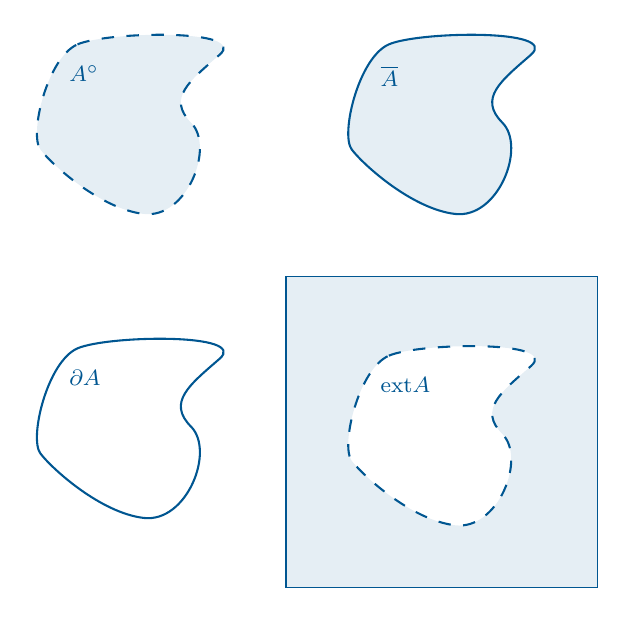
\begin{tikzpicture}[x=0.75pt,y=0.75pt,yscale=-1,xscale=1]
	%uncomment if require: \path (0,300); %set diagram left start at 0, and has height of 300

	%Shape: Polygon Curved [id:ds678130924119981] 
	\draw  [color={rgb, 255:red, 0; green, 86; blue, 145 }  ,draw opacity=1 ][fill={rgb, 255:red, 0; green, 86; blue, 145 }  ,fill opacity=0.1 ][dash pattern={on 4.5pt off 4.5pt}][line width=0.75]  (49.56,38.17) .. controls (64.04,31.89) and (132.48,30.63) .. (118,43.2) .. controls (103.53,55.77) and (92.59,64.15) .. (104.25,75.88) .. controls (115.91,87.61) and (102.23,122.38) .. (81.41,119.87) .. controls (60.58,117.36) and (37.36,96.23) .. (31.71,88.87) .. controls (26.05,81.5) and (35.08,44.45) .. (49.56,38.17) -- cycle ;
	%Shape: Polygon Curved [id:ds19735692429512375] 
	\draw  [color={rgb, 255:red, 0; green, 86; blue, 145 }  ,draw opacity=1 ][fill={rgb, 255:red, 0; green, 86; blue, 145 }  ,fill opacity=0.1 ][line width=0.75]  (199.56,38.17) .. controls (214.04,31.89) and (282.48,30.63) .. (268,43.2) .. controls (253.53,55.77) and (242.59,64.15) .. (254.25,75.88) .. controls (265.91,87.61) and (252.23,122.38) .. (231.41,119.87) .. controls (210.58,117.36) and (187.36,96.23) .. (181.71,88.87) .. controls (176.05,81.5) and (185.08,44.45) .. (199.56,38.17) -- cycle ;
	%Shape: Polygon Curved [id:ds4025351553833618] 
	\draw  [color={rgb, 255:red, 0; green, 86; blue, 145 }  ,draw opacity=1 ][line width=0.75]  (49.56,184.63) .. controls (64.04,178.34) and (132.48,177.09) .. (118,189.66) .. controls (103.53,202.23) and (92.59,210.6) .. (104.25,222.34) .. controls (115.91,234.07) and (102.23,268.84) .. (81.41,266.33) .. controls (60.58,263.82) and (37.36,242.69) .. (31.71,235.32) .. controls (26.05,227.96) and (35.08,190.91) .. (49.56,184.63) -- cycle ;
	%Shape: Path Data [id:dp28607428735171037] 
	\draw  [draw opacity=0][fill={rgb, 255:red, 0; green, 86; blue, 145 }  ,fill opacity=0.1 ][dash pattern={on 4.5pt off 4.5pt}] (300,150) -- (300,300) -- (150,300) -- (150,150) -- (300,150) -- cycle (199.56,188.17) .. controls (185.08,194.45) and (176.05,231.5) .. (181.71,238.87) .. controls (187.36,246.23) and (210.58,267.36) .. (231.41,269.87) .. controls (252.23,272.38) and (265.91,237.61) .. (254.25,225.88) .. controls (242.59,214.15) and (253.53,205.77) .. (268,193.2) .. controls (282.48,180.63) and (214.04,181.89) .. (199.56,188.17) -- cycle ;
	%Shape: Square [id:dp6423377198062709] 
	\draw  [color={rgb, 255:red, 0; green, 86; blue, 145 }  ,draw opacity=1 ] (150,150) -- (300,150) -- (300,300) -- (150,300) -- cycle ;
	%Shape: Polygon Curved [id:ds7262645597364767] 
	\draw  [color={rgb, 255:red, 0; green, 86; blue, 145 }  ,draw opacity=1 ][dash pattern={on 4.5pt off 4.5pt}][line width=0.75]  (199.56,188.17) .. controls (214.04,181.89) and (282.48,180.63) .. (268,193.2) .. controls (253.53,205.77) and (242.59,214.15) .. (254.25,225.88) .. controls (265.91,237.61) and (252.23,272.38) .. (231.41,269.87) .. controls (210.58,267.36) and (187.36,246.23) .. (181.71,238.87) .. controls (176.05,231.5) and (185.08,194.45) .. (199.56,188.17) -- cycle ;

	% Text Node
	\draw (44.33,47.33) node [anchor=north west][inner sep=0.75pt]  [font=\footnotesize,color={rgb, 255:red, 0; green, 86; blue, 145 }  ,opacity=1 ]  {$A^{\circ }$};
	% Text Node
	\draw (194.33,47.33) node [anchor=north west][inner sep=0.75pt]  [font=\footnotesize,color={rgb, 255:red, 0; green, 86; blue, 145 }  ,opacity=1 ]  {$\overline{A}$};
	% Text Node
	\draw (44.33,193.79) node [anchor=north west][inner sep=0.75pt]  [font=\footnotesize,color={rgb, 255:red, 0; green, 86; blue, 145 }  ,opacity=1 ]  {$\partial A$};
	% Text Node
	\draw (194.33,197.33) node [anchor=north west][inner sep=0.75pt]  [font=\footnotesize,color={rgb, 255:red, 0; green, 86; blue, 145 }  ,opacity=1 ]  {$\mathrm{ext} A$};


\end{tikzpicture}
